\documentclass[main]{subfiles}
\begin{document}

\section*{Lecture 15 // Oct. 13 // Cobordism Maps}
\addcontentsline{toc}{section}{Lecture 15 -- Cobordism Maps}

\begin{recall}
Given a cobordism $W$ from $Y_1$ to $Y_2$, we defined
\[
\mc{M}_{[\gamma]}(x,W^\ast,y) = \left\{\begin{array}{l}\text{ASD conn. on } W^\ast \\ \text{limiting to } x,y \\ \text{in component } \gamma\end{array}\right\}\Big/\text{gauge}
\]
Note that there are $\mathbb{Z}$-many components.
\end{recall}

Today, we'll continue defining the chain maps induced by $W$.

We'll restrict cobordisms $W$ to those which satisfy $b_2^+(W)=b_1(W)=0$. Let's define a grading-preserving chain map $F_W$ in the $C$, $\overline{C}$, and $\underline{C}$ settings.

\begin{definition}[$F_W$ for the irreducible complex]
Take $x\in C(Y_1)$.
\[
F_W(x) := \lambda(x) = \sum_{y\in C(Y_2)}\ \sum_{\substack{\gamma \\ \dim(\mc{M}_\gamma)=0}} \#\mc{M}_\gamma(x,W^\ast,y)\, y.
\]
Note that unlike for $Y^3\times\mathbb{R}$, $W$ has no $\mathbb{R}$-action, so we don't quotient by $\mathbb{R}$.
\end{definition}

\begin{claim}
$F_W$ is a chain map: $F_W\circ\partial_{Y_1} = \partial_{Y_2}\circ F_W$.
\end{claim}

\begin{proof}
Exercise.
\end{proof}

The more interesting definitions are those for the upper and lower bar complexes. Recall that $\overline{C}$ is formed from the irreducible complex by incorporating flows into the reducible. We take $C$ and add a copy of the field we're working in at grading $0$, viewing it as the generator corresponding to $\Theta$: $\overline{C} = C\oplus\mathbb{F}_{(0)}$. The differential is $\overline{\partial}=\partial+D_1$, and it's convenient to view $\overline{\partial}$ as having components, e.g.,
\[
\overline{\partial} = \begin{bmatrix}\partial & 0\\ D_1 & 0\end{bmatrix}.
\]
The upper right entry is $0$, since by definition of $\overline{C}$, there are no maps from reducible components to irreducibles. The lower right entry is zero since the differential of the reducible can't be supported on the reducible, since the differential drops the grading by one.

To define $F_W$ in the $\overline{C}$-context, we'll also define it on components. For simplicity, assume that $H_1(W;\mathbb{Z})=0$. Then $F_W : \overline{C}(Y_1)\to\overline{C}(Y_2)$ is given by
\[
F_W = \begin{bmatrix}\lambda & 0\\ \Delta & 1\end{bmatrix},
\]
where
\begin{itemize}
\item[] $\lambda$: Irreducible generators $\to$ Irreducible generators
\item[] $\Delta_1$: Irreducible generators $\to$ Reducible generators
\item[] $1$: Reducible generators $\to$ Reducible generators
\item[] $0$: Reducible generators $\to$ Irreducible generators
\end{itemize}
This motivates the following formal definition.

\begin{definition}[$F_W$ for $\overline{C}$]
When $H_1(W;\mathbb{Z})=0$,
\[
F_W(x) = \begin{bmatrix}\lambda & 0\\ \Delta & 1\end{bmatrix}(x), \quad \text{where } x\in C\oplus\mathbb{F}_{(0)},
\]
\[
\lambda(x) = \sum_{y\in C(Y_2)}\ \sum_{\substack{\gamma \\ \dim(\mc{M}_\gamma)=0}} \#\mc{M}_\gamma(x,W^\ast,y)\, y \quad \text{as before,}
\]
\[
\Delta_1(x) = \sum_{\substack{\gamma \\ \dim(\mc{M}_\gamma)=0}} \#\mc{M}_\gamma(x,W^\ast,\Theta)\,\Theta,
\]
and the one in the lower right represents the obvious trivial connection on $W^\ast$.

In general, when $H_1(W;\mathbb{Z})\neq 0$, $F_W$ is defined to have components
\[
F_W = \begin{bmatrix}\lambda & 0\\ \Delta_1 & c\end{bmatrix} \quad \text{where } c = |H_1(W;\mathbb{Z})|.
\]
\end{definition}

The $1$ (or $c$) from reducibles to reducibles can be viewed more explicitly. When $H_1=0$, pick the trivial bundle on $W^\ast$ agreeing with the trivial bundles on each end. The $0$ connection on each end and this trivialization defines a $0$ connection over all of $W^\ast$, which clearly sends $\Theta$ to $\Theta$. When $H_1\neq 0$, this component also roughly has the interpretation as counting ASD connections going from $\Theta$ to $\Theta$, but it turns out that there are $H_1$-many reducible flat connections over $W^\ast$.

\begin{claim}
$F_W\circ\overline{\partial} = \overline{\partial}\circ F_W$.
\end{claim}

\begin{proof}
Exercise.
\end{proof}

\begin{remark}
The map $\lambda$ can be thought of like the $D_1$ map by replacing $W$ with $Y\times\mathbb{R}$ and quotienting by $\mathbb{R}$.
\end{remark}

Of course the $\underline{C}$ complex is very similar to that of $\overline{C}$: we disallow flows into $\Theta$, but allow those out of $\Theta$.

\begin{definition}[$F_W$ for $\underline{C}$]
\[
\underline{C} = C\oplus\mathbb{F}_{(-3)}
\]
\[
\underline{\partial} = \partial+D_2 = \begin{pmatrix}\partial & D_2\\ 0 & 0\end{pmatrix}
\]
\[
F_W = \begin{pmatrix}\lambda & \Delta_2\\ 0 & c\end{pmatrix}
\]
where $\lambda, c$ are as before and
\[
\Delta_2(\Theta) = \sum_{y\in C(Y_2)}\ \sum_{\substack{\gamma \\ \dim=0}} \#\mc{M}_\gamma(\Theta,W^\ast,y)\, y.
\]
\end{definition}

We now ask: What does this formalism buy us?

\subsection*{Obstructing Cobordisms}

Let's work with the underbar complex, $\underline{C}$. We can also think about the $D_2$ map as giving us the information of a particular class of the irreducible complex $C(Y)$. We'll call $D_2(\Theta)$ the ``$D_2$-class'', e.g., $[D_2^Y]:=[D_2(\Theta)]=[D_2(1)]$. The (rather boring) observation is that a negative-definite $b_1=0$ cobordism $W$ scales the $D_2$-class by $c$.

\begin{theorem}
Let $W$ be a negative definite $b_1=0$ cobordism from $Y_1$ to $Y_2$. Set $c=|H_1(W;\mathbb{Z})|$. Then
\[
F_W[D_2^{Y_1}] = c[D_2^{Y_2}].
\]
\end{theorem}

\begin{proof}
Consider the following complexes for $Y_1,Y_2$.
\begin{center}
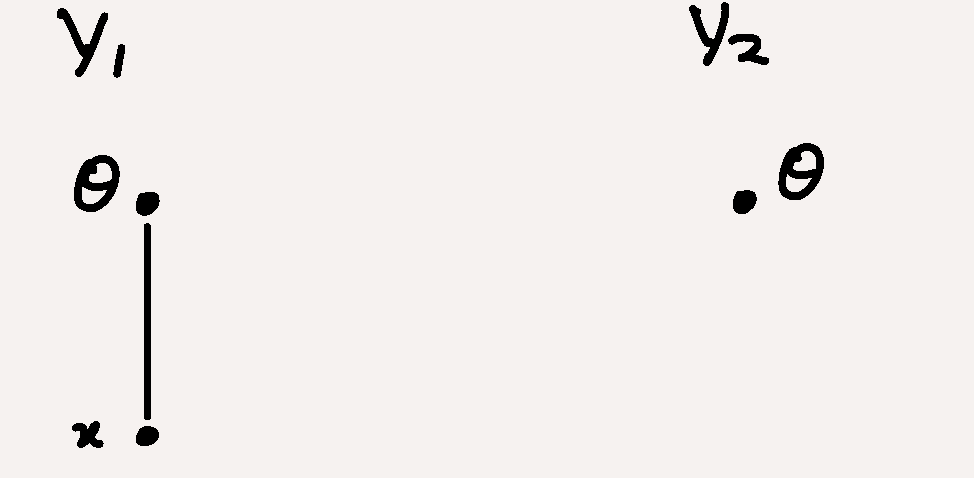
\includegraphics[width=0.4\linewidth]{figures/fig_lec15_complexes.png}
\end{center}

Since reducibles must map to reducibles, there must be an arrow like so
\begin{center}
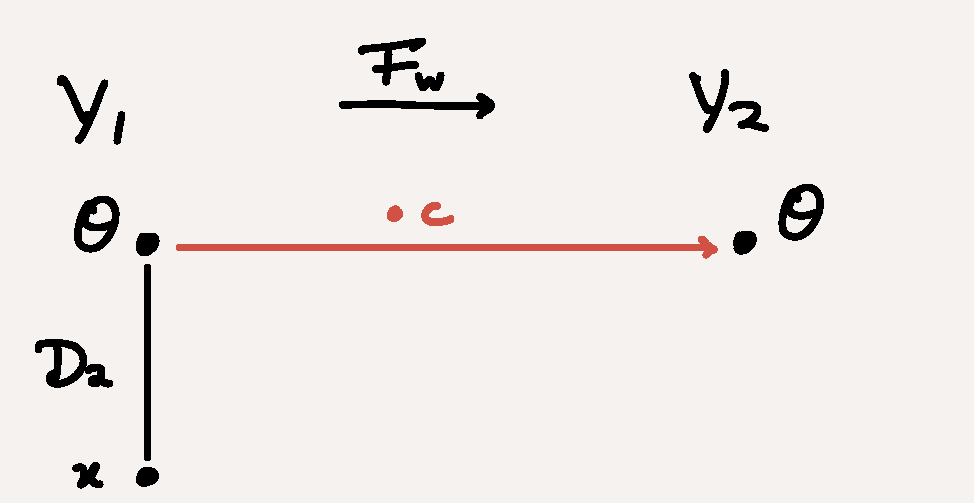
\includegraphics[width=0.45\linewidth]{figures/fig_lec15_arrow_c.png}
\end{center}

Note that this is related to the question from last time: why define $\underline{C}$ and $\overline{C}$? It's these definitions that give us the map $c$ from reducibles to reducibles, so we know there is an arrow.

There might be other arrows and other generators, but we've asserted that $F_W$ is a chain map, so $F_W(x)$ must also multiply by $c$.
\begin{center}
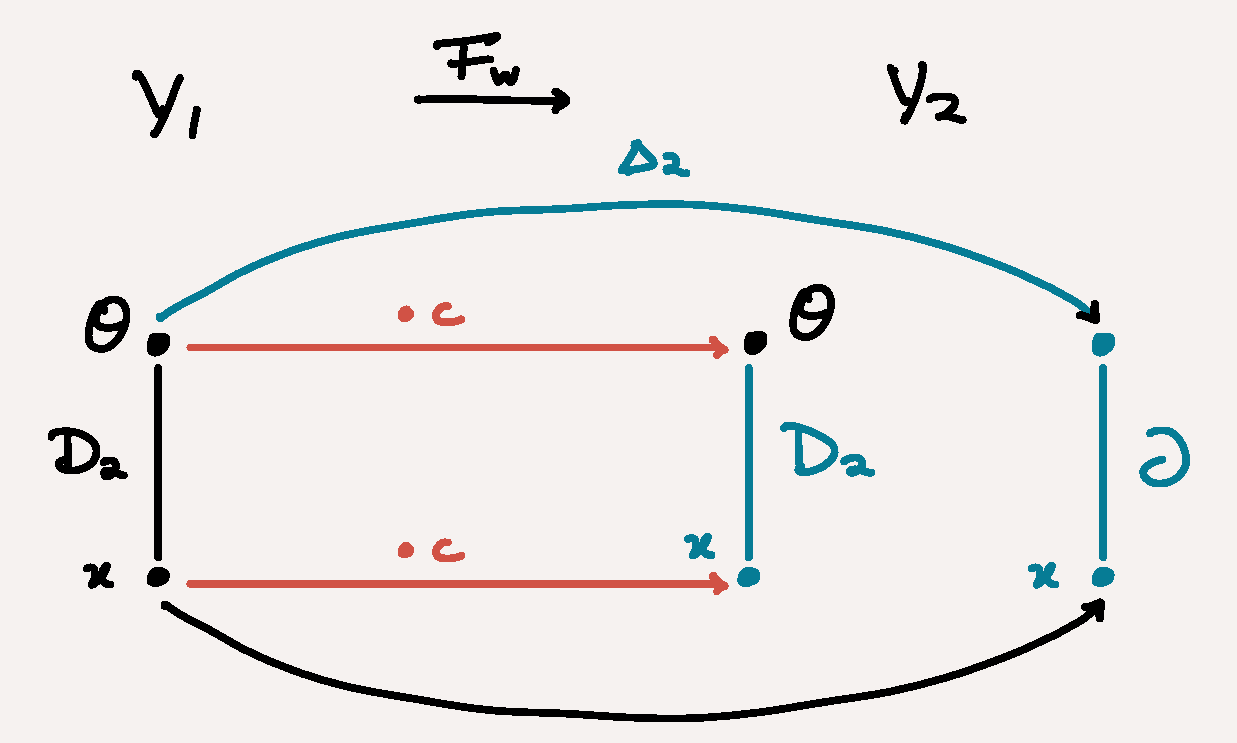
\includegraphics[width=0.7\linewidth]{figures/fig_lec15_chain_map.png}
\end{center}

Formally,
\begin{align*}
(F_W\circ\underline{\partial})(\Theta) &= (\underline{\partial}\circ F_W)(\Theta)\\
F_W(D_2(\Theta)) &= (\underline{\partial}\circ F_W)(\Theta)\\
&= (\partial+D_2)(F_W(\Theta))\\
&= (\partial+D_2)(c\Theta+\Delta_2\Theta)\\
&= \partial(c\Theta)+D_2(c\Theta)+\partial(\Delta_2\Theta)+D_2(\Delta_2\Theta)\\
&= cD_2\Theta+\partial(\Delta_2\Theta)
\end{align*}
since $\partial(c\Theta)=0$ and $D_2(\Delta_2\Theta)=0$. ($c$ is the constant map, so $D_2(c\Theta)=cD_2\Theta$.) \qedhere
\end{proof}

Note that it's instructive to write out what $\underline{\partial}\circ F_W = F_W\circ\underline{\partial}$ actually means:
\[
\begin{pmatrix}\partial & D_2\\ 0 & 0\end{pmatrix}\begin{pmatrix}\lambda & \Delta_2\\ 0 & c\end{pmatrix} = \begin{pmatrix}\lambda & \Delta_2\\ 0 & c\end{pmatrix}\begin{pmatrix}\partial & D_2\\ 0 & 0\end{pmatrix}
\]
\[
\begin{bmatrix}\partial\lambda & \partial\Delta_2+D_2c\\ 0 & 0\end{bmatrix} = \begin{bmatrix}\lambda\partial & \lambda D_2\\ 0 & 0\end{bmatrix}
\]
so this equality implies a more complex relationship between the maps $\partial, D_2,\lambda,\Delta_2,c$.

As a consequence, we can obstruct cobordisms by calculating $D_2$ maps.

\begin{corollary}
If $[D_2^{Y_1}]=0$ but $[D_2^{Y_2}]\neq 0$, then there does not exist a negative-definite $b_1=0$ cobordism $W$ from $Y_1$ to $Y_2$.
\end{corollary}

Intuitively, cobordism maps take ``red to red'', i.e., $\Theta\mapsto c\Theta+(\text{other stuff})$. Therefore, there can be no situation where $\Theta$ maps to nothing but $F_W(\Theta)$ does map to something:
\begin{center}
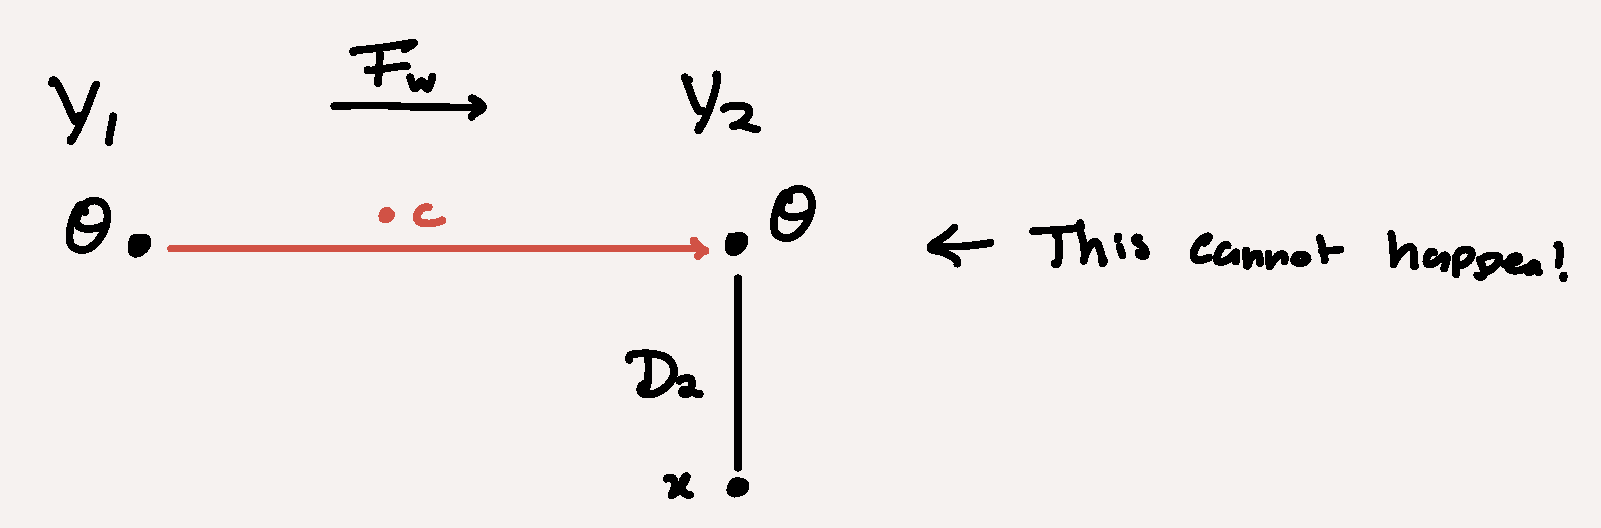
\includegraphics[width=0.6\linewidth]{figures/fig_lec15_cannot_happen.png}
\end{center}
However, the claim is not that $D_2=0$, but $[D_2]=0$, so it is o.k.\ for the complex to look like this:
\begin{center}
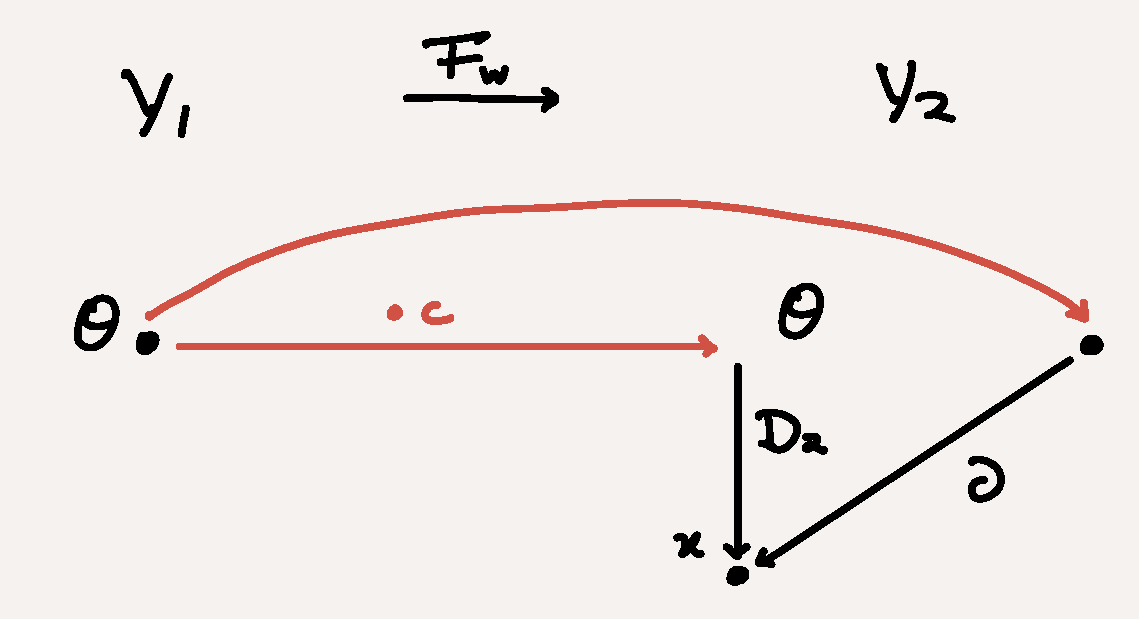
\includegraphics[width=0.5\linewidth]{figures/fig_lec15_ok_complex.png}
\end{center}

This is the ethos of Floer theory: say some cobordism map has some formal property, then show that there does not exist any map with that property.

\begin{remark}
\begin{enumerate}
\item This is analogous to the $d$-invariant being a particular sign (there is a more precise statement of this).
\item $D_1$ gives a cohomology class. Roles of $Y_1,Y_2$ will switch.
\item Just like for the differentials, all cobordism maps lift to the $\mathbb{Z}$-version.
\end{enumerate}
\end{remark}

So far, this discussion is very similar to other Floer homologies. IFH is special because it admits a filtration by CS value; we have not used that yet in this discussion.

\subsection*{Cobordism Maps \& the CS Filtration}

The overarching claim here is that everything we've seen so far is actually filtered.

\begin{theorem}
$F_W$ is filtered.
\end{theorem}

\begin{proof}
If $y$ appears in $F_W(x)$, then there is some ASD connection $A$ limiting to $x$ and $y$ on the ends. This can be thought of as ``$A$ restricts to $x$ and $y$ on each boundary'', but this is slightly false; the analysis prefers open boundaries to fixed conditions on closed boundaries.

Then, again playing fast and loose with orientations, we get that
\begin{align*}
\widetilde{\CS}(y)-\widetilde{\CS}(x) &= \frac{1}{8\pi^2}\int_W\tr(F_A\wedge F_A)\\
&= \frac{-1}{8\pi^2}\int_W\tr(F_A\wedge\ast F_A)\\
&= -\|F_A\|_{L^2}^2\ \leq\ 0.
\end{align*}
Thus $\widetilde{\CS}(y)\leq\widetilde{\CS}(x)$. \qedhere
\end{proof}

So $F_W$ is filtered exactly because the CS functional is a norm.

\begin{theorem}
Suppose $x,y$ correspond to $\SU(2)$-representations of $\pi_1(Y_1)$ and $\pi_1(Y_2)$. If $y$ appears in $F_W(x)$ and $\widetilde{\CS}(x)=\widetilde{\CS}(y)$, then there exists an $\SU(2)$ representation of $\pi_1(W)$ which restricts to that of $x$ and $y$. E.g., given representations $\rho_1:\pi_1(Y_1)\to\SU(2)$ and $\rho_2:\pi_1(Y_2)\to\SU(2)$, there is a representation $\rho:\pi_1(W)\to\SU(2)$ such that $\rho|_{\pi_1(Y_i)}=\rho_i$.
\end{theorem}

\begin{proof}
If $\widetilde{\CS}(x)=\widetilde{\CS}(y)$, $-\|F_A\|_{L^2}^2=0$, so $A$ has no curvature, and defines a representation of $\pi_1(W)$. \qedhere
\end{proof}

The obvious takeaway is that the cobordism map on IFH is affected by $\pi_1$ of the cobordism. But what this is actually saying is subtle: the very existence of cobordisms is determined by representations of $\pi_1$. This gives the following corollary.

\begin{corollary}
If $\pi_1(W)=1$, then $F_W$ is strictly filtered except for the $\Theta$-to-$\Theta$ component.
\end{corollary}

Again, so what? We actually have enough formal properties to conclude our first application! Recall that on the first day, we asked whether the Poincar\'e homology sphere $\Sigma(2,3,5)$ admits a simply connected self-homology cobordism. We claimed that this was an interesting question, since it's equivalent to asking whether $\Sigma(2,3,5)\#-\Sigma(2,3,5)$ bounds a simply connected homology ball. The underlying question is: does every $\mathbb{Z}\mathrm{HS}^3$ bound a contractible $\mathbb{Z}\mathrm{HB}^4$?

The point here is that instantons can detect this, in this subtle way. Let's look at the IFH of the Poincar\'e sphere. This does, unfortunately, open the can of worms which asks how does one compute this? But we'll punt this question to later.

\begin{example}\label{ex:sigma235}
Instanton Floer complex of $\Sigma(2,3,5)$:
\begin{center}
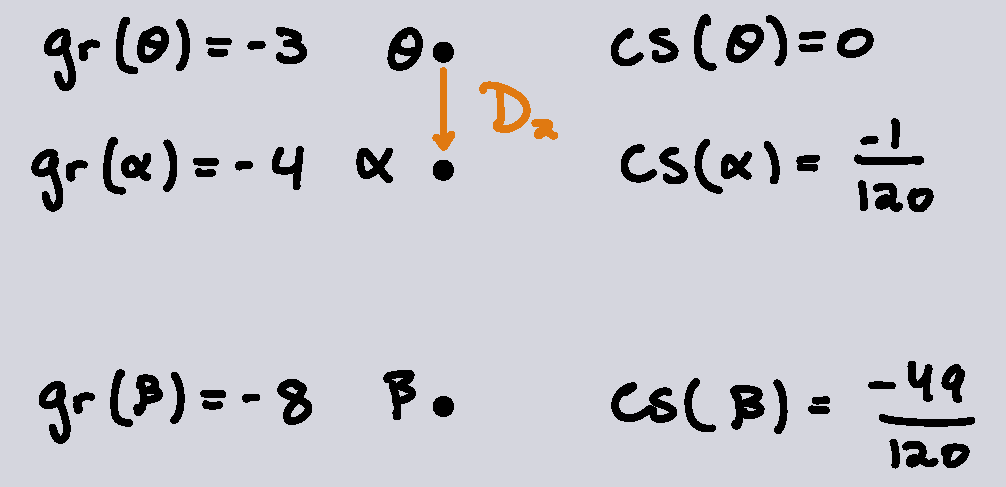
\includegraphics[width=0.55\linewidth]{figures/fig_lec15_example_complex.png}
\end{center}

Is it possible that there is a $\pi_1=1$ self-homology cobordism? If so, it induces a cobordism map. Since $H_1=0$, $\Theta\mapsto\Theta$, and since $F_W$ commutes with $D_2$, $\alpha\mapsto\alpha$. However, sending $\alpha$ to itself is not strictly filtered.
\begin{center}
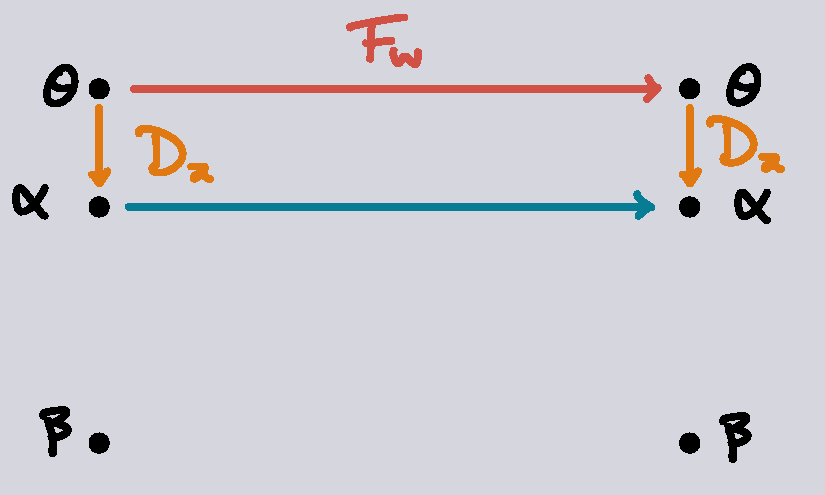
\includegraphics[width=0.4\linewidth]{figures/fig_lec15_no_filtered.png}
\end{center}
Therefore $W$ cannot be simply connected.
\end{example}

It is important here that we knew something about the $D_2$ map. If we didn't know about $\Theta$, there's no reason why $F_W$ can't be $0$. But $\Theta$ tells us that $\Theta\mapsto\Theta$, so this ``shadow'' of the $D_2$ map forces $\alpha\mapsto\alpha$. This is actually a completely general fact.

\begin{theorem}
If $[D_2^Y]\neq 0$, then there does not exist any simply connected homology cobordism from $Y$ to $Y$.
\end{theorem}

\begin{proof}
Choose a representative of $[D_2^Y]$ in $H_\ast(C(Y))$ with minimal CS filtration. (The filtration of the chain complex induces a filtration on $H_\ast$.) This element can be written as $\sum_i c_ix_i\in H_\ast(C(Y))$, and $\mathrm{filt}\left(\sum_i c_ix_i\right)=\max\mathrm{filt}(x_i)$, so
\[
\mathrm{filt}([x]) = \min\ \mathrm{filt.\ of\ representatives\ of\ }[x].
\]
If there was a simply connected homology cobordism $W:Y\to Y$, then $\mathrm{filt}(F_W(x))<\mathrm{filt}(x)$. But $F_W(x)$ is also a representative of $[D_2^Y]$, implying our original choice for $x$ was not minimal. $\Rightarrow\Leftarrow$ \qedhere
\end{proof}

So ``most'' things don't admit simply connected self-homology cobordisms.

\end{document}
